\documentclass{jsarticle}
\usepackage{amsmath, smssymb, amsfonts}
\usepackage{newtxtext, newtxmath}
\usepackage{latexsym}
\usepackage{mathrsfs}
\usepackage{mathtools}
\usepackage{textcomp}
\usepackage{mathcomp}
\usepackage[dvipdfmx]{graphicx, xcolor}
\usepackage{float}
\usepackage{wrapfig}	% must be after float package.
\usepackage{subcaption}
\usepackage{booktabs}
\usepackage{url}
\usepackage{listings, jvlisting, color}

\definecolor{OliveGreen}{rgb}{0.0,0.6,0.0}
\definecolor{Orenge}{rgb}{0.89,0.55,0}
\definecolor{SkyBlue}{rgb}{0.28, 0.28, 0.95}
\lstset{
  language={C++}, % 言語の指定
  basicstyle={\ttfamily},
  identifierstyle={\small},
  commentstyle={\smallitshape},
  keywordstyle={\small\bfseries},
  ndkeywordstyle={\small},
  stringstyle={\small\ttfamily},
  frame={tb},
  breaklines=true,
  columns=[l]{fullflexible},
  numbers=left,
  xrightmargin=0zw,
  xleftmargin=3zw,
  numberstyle={\scriptsize},
  stepnumber=1,
  numbersep=1zw,
  lineskip=-0.5ex,
  keywordstyle={\color{SkyBlue}},     %キーワード(int, ifなど)の書体指定
  commentstyle={\color{OliveGreen}},  %注釈の書体
  stringstyle=\color{Orenge}          %文字列
}


\begin{document}

\title{ゼミ レポート07}
\author{山田朔也}
\maketitle

\section{本レポートについて}
本レポートは6月14日に行われたゼミにて出題された課題に対するレポートとなっている。
課題の内容は、前回のレポートで計算した1次元磁膜を2次元に拡張することとなる。

\section{原理}
\subsection{2次元Bloch磁壁}
2次元では、膜の表面付近で磁気モーメントが膜面に平行な方向を向くことにより、
膜の表面に現れる磁極が減少し、静磁エネルギーが減少させることができる。
よって、2次元のBloch磁壁の磁化構造は図\ref{fig01}で表される。
\begin{figure}[H]
	\centering
	\begin{subfigure}{0.49\columnwidth}
		\centering
		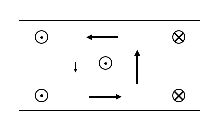
\includegraphics[width=\columnwidth]{pic05.eps}
		\caption{非対称Bloch磁壁}
		\label{fig01_1}
	\end{subfigure}
	\begin{subfigure}{0.49\columnwidth}
		\centering
		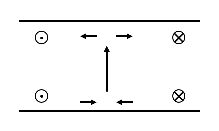
\includegraphics[width=\columnwidth]{pic06.eps}
		\caption{2次元対称Bloch磁壁}
		\label{fig01_2}
	\end{subfigure}
	\caption{2次元Bloch磁壁の磁化構造の概念図}
	\label{fig01}
\end{figure}

\subsection{2次元$\mathrm{N\Acute{e}el}$磁壁}
2次元$\mathrm{N\Acute{e}el}$磁壁の磁化構造とその周りに発生する磁極は
図\ref{fig02}で表される。
\begin{figure}[H]
	\centering
	\begin{subfigure}{0.49\columnwidth}
		\centering
		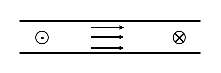
\includegraphics[width=\columnwidth]{pic07.eps}
		\caption{対称$\mathrm{N\Acute{e}el}$磁壁}
		\label{fig02_1}
	\end{subfigure}
	\begin{subfigure}{0.49\columnwidth}
		\centering
		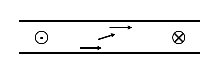
\includegraphics[width=\columnwidth]{pic08.eps}
		\caption{非対称$\mathrm{N\Acute{e}el}$磁壁}
		\label{fig02_2}
	\end{subfigure}
	\caption{2次元$\mathrm{N\Acute{e}el}$磁壁の磁化構造の概念図}
	\label{fig02}
\end{figure}

なお、非対称$\mathrm{N\Acute{e}el}$磁壁は、対称$\mathrm{N\Acute{e}el}$磁壁が発生する条件より
さらに膜厚を厚くしていくと現れる。
ただし、厚くしすぎるとBloch磁壁が現れる。

\subsection{自由境界条件}
2次元磁壁の磁化構造を求める場合、$\pm \mathrm{x}$の境界領域はディレクレ条件を用い、
$\pm \mathrm{z}$の境界領域はノイマン条件を用いる。

ノイマン条件は、境界上で次の関係を満たすように磁気モーメントの向きを設定する。
\begin{equation}
	\frac{d\vec{M}}{dn} = 0
\end{equation}
ここでnは境界領域での法線方向となる。

今回の計算では、計算領域の外に仮想的に0番目の計算セルを想定し、その位置での磁気モーメントの向きと、
1番目のセルの磁気モーメントの向きを用いて、式\ref{01}の関係が成り立つようにする。
\begin{equation}
	\frac{\delta \vec{M}}{\delta z} = \frac{\vec{M_1} - \vec{M_0}}{dz} = 0
	\label{01}
\end{equation}

この式より、計算領域の外の仮想セルでの磁気モーメントの向きは、
計算領域の端の点での向きと同じものを設定すれば良いことが分かる。

\section{問題}
\subsection{問題内容}
問題内容は、膜厚方向の磁化構造も考慮した2次元計算を行う。
その上で、以下の内容を調べる。
\begin{enumerate}
	\item 2次元計算での静磁界係数式を導出する。
	\item 静磁界係数を求めるプログラムを作成し、対称性を調べる。
	\item 2次元のBloch磁壁及び$\mathrm{N\Acute{e}el}$磁壁の磁化構造を求め、得られた磁化構造を図で示す。
	\item 計算点と計算時間の関係をグラフで示す。
\end{enumerate}
上記の項目をそれぞれ小問1-4として回答をしていく。

\subsection{材料定数等}
材料定数等は、各小問の欄で特筆しない限り以下のものを使用する。
\begin{itemize}
	\item 飽和磁化$M = 800\;\mathrm{emu/cm^3}$
	\item 交換スティフネス定数$A = 1\times 10^{-6}\;\mathrm{erg/cm}$
	\item 異方性定数$K_u = 0\;\mathrm{erg/cm^3}$
	\item 損失定数$\alpha = 1$
	\item 磁気回転比$\lvert\gamma\rvert = 1.76\times 10^7\;\mathrm{rad/(s\cdot Oe)}$
	\item 時間刻み$\mathrm{dt} = 0.1\times 10^{-12}\;\mathrm{s}$
	\item 格子間隔$\mathrm{dx} = 80\;$\AA
	\item 格子間隔$\mathrm{dz} = 80\;$\AA
	\item x方向の計算点数$\mathrm{nx} = 30$
	\item z方向の計算点数$\mathrm{nz} = 20$
	\item x方向の境界領域では、ディレクレ条件を用い、左端を(0,-1,0)、右端を(0,1,0)とする。
	\item z方向の境界領域では、ノイマン条件を用いる。
	\item 初期値(非対称Bloch磁壁):
	\begin{itemize}
		\item 膜表面:図\ref{fig01_1}に示した表面付近の磁化構造
		\item 表面以外:1次元Bloch磁壁の計算で用いたもの
	\end{itemize}
	\item 初期値(対称Bloch磁壁):
	\begin{itemize}
		\item 膜表面:図\ref{fig01_2}に示した表面付近の磁化構造
		\item 表面以外:1次元Bloch磁壁の計算で用いたもの
	\end{itemize}
	\item 初期値(非対称$\mathrm{N\Acute{e}el}$磁壁):
	\begin{itemize}
		\item 膜表面:1次元$\mathrm{N\Acute{e}el}$磁壁の計算で用いたもの
		\item 表面以外:mx,myをそれぞれ0.1に設定
	\end{itemize}
	\item 初期値(対称$\mathrm{N\Acute{e}el}$磁壁):1次元$\mathrm{N\Acute{e}el}$磁壁の計算で用いたもの
\end{itemize}

\subsection{小問1}
この問題では、2次元計算での静磁界係数を導出する。

まず、静磁界は、z軸に平行な辺が作る磁界と、x軸に平行な辺が作る磁界のふたつあり、それぞれ式\ref{05},\ref{06},\ref{07},\ref{08}で表された。
\begin{align}
	Hx = &-2Mx\left(\tan^{-1}\frac{z1}{x1} - \tan^{-1}\frac{z1}{x0} - \tan^{-1}\frac{z0}{x1} + \tan^{-1}\frac{z0}{x0}\right) = qxx\cdot mx	\label{05} \\
		 &\left(\text{但し}\frac{z1}{x1},\frac{z1}{x0},\frac{z0}{x1},\frac{z0}{x0} \text{は} -\frac{2}{\pi} \text{から} \frac{2}{\pi} \text{の値} \right) \notag \\
	Hz = &-Mx\left[\log\left(x1^2+z1^2\right) - \log\left(x1^2+z0^2\right) - \log\left(x0^2+z1^2\right) + \log\left(x0^2+z0^2\right)\right] = qxz\cdot mx	\label{06}
\end{align}
\begin{align}
	Hz &= -2Mz\left(\tan^{-1}\frac{x1}{z1} - \tan^{-1}\frac{x1}{z0} - \tan^{-1}\frac{x0}{z1} + \tan^{-1}\frac{x0}{z0}\right) = qzz\cdot mz	\label{07} \\
	Hx &= -Mz\left[\log\left(z1^2+x1^2\right) - \log\left(z1^2+x0^2\right) - \log\left(z0^2+x1^2\right) + \log\left(z0^2+x0^2\right)\right] \notag \\
	   &= qzx\cdot mz = qxz\cdot mz	\label{08}
\end{align}
これらの式を、まとめることで式\ref{09},\ref{10}として表される。
\begin{equation}
	Hx = qxx\cdot mx + qxz\cdot mz
	\label{09}
\end{equation}
\begin{equation}
	Hz = qxz\cdot mx + qzz\cdot mz
	\label{10}
\end{equation}

ここで、今回は前回と異なり、計算セルが2次元方向に存在しているため、
それを踏まえて考えるとqxx,qzz,qxzはそれぞれ式\ref{11},\ref{12},\ref{13}で表される。
\begin{alignat}{2}
	&qxx(k,l) &= &-2M\left( \tan^{-1}\frac{(l+0.5)dz}{(k+0.5)dx} - \tan^{-1}\frac{(l+0.5)dz}{(k-0.5)dx} - \tan^{-1}\frac{(l-0.5)dz}{(k+0.5)dx} + \tan^{-1}\frac{(l-0.5)dz}{(k-0.5)dx} \right)	\label{11} \\
	&qzz(k,l) &= &-2M\left( \tan^{-1}\frac{(k+0.5)dx}{(l+0.5)dz} - \tan^{-1}\frac{(k-0.5)dx}{(l+0.5)dz} - \tan^{-1}\frac{(k+0.5)dx}{(l-0.5)dz} + \tan^{-1}\frac{(k-0.5)dx}{(l-0.5)dz} \right)	\label{12} \\
	&qxz(k,l) &= &-M\log\left[ \{(k+0.5)dx\}^2 + ((l+0.5)dz)^2 \right] + M\log\left[ \{(k-0.5)dx\}^2 + ((l+0.5)dz)^2 \right]	\notag \\
			 &&&+M\log\left[ \{(k+0.5)dx\}^2 + ((l-0.5)dz)^2 \right] - M\log\left[ \{(k-0.5)dx\}^2 + ((l-0.5)dz)^2 \right] \qquad (=0)	\label{13}
\end{alignat}

ここで、kはx方向の番目を表し、lはz方向の番目を表す。

\subsection{小問2}
この問題では、静磁界係数を求めるプログラムを作成し、対称性を調べる。
まずは式\ref{11},\ref{12},\ref{13}で表されるqxx,qzz,qxzの計算結果を、表\ref{fig03}にまとめた。
ただし、$\mathrm{nx}=4,\;\mathrm{nd}=2$として計算は行った。
\begin{figure}[H]
	\centering
	\begin{subfigure}{0.8\columnwidth}
		\centering
		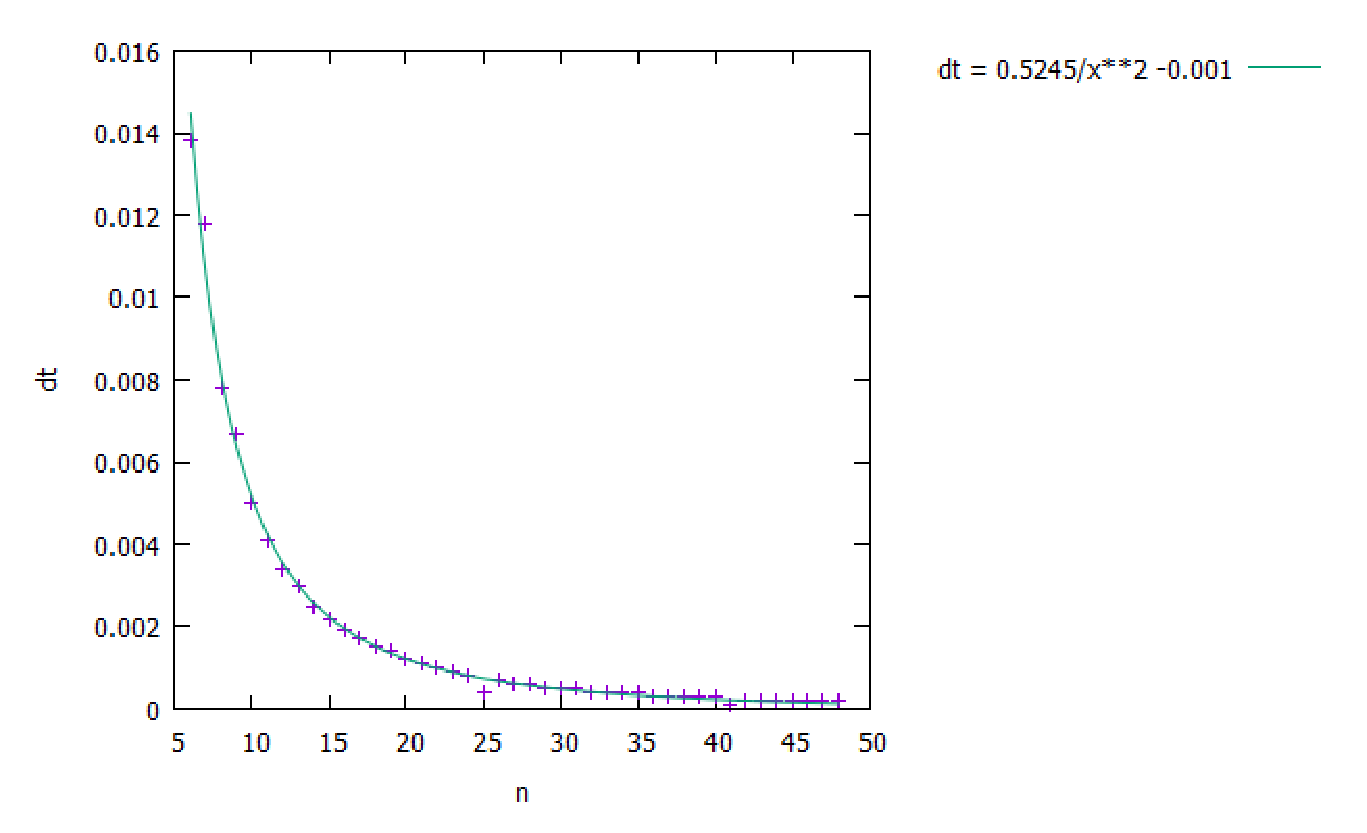
\includegraphics[width=\columnwidth]{pic09.eps}
		\caption{qxxの計算結果}
		\label{fig03_1}
	\end{subfigure}
	\begin{subfigure}{0.8\columnwidth}
		\centering
		\includegraphics[width=\columnwidth]{pic10.eps}
		\caption{qzzの計算結果}
		\label{fig03_2}
	\end{subfigure}
	\begin{subfigure}{0.8\columnwidth}
		\centering
		\includegraphics[width=\columnwidth]{pic10.eps}
		\caption{qxzの計算結果}
		\label{fig03_3}
	\end{subfigure}
	\caption{静磁界係数の計算結果}
	\label{fig03}
\end{figure}

表\ref{fig03}から、qxx,qzzは$\mathrm{k,l}=0$を中心として対称となった。
またqxzは同じく中心を対称としているが、正負が逆転するという結果となった。

\subsection{小問3}
この小問では、2次元のBloch磁壁及び$\mathrm{N\Acute{e}el}$磁壁の磁化構造を求め、得られた磁化構造を図で示す。

ただし、$\mathrm{N\Acute{e}el}$磁壁では$\mathrm{nz}=6$として計算した。

計算結果の図は、gnuplotのベクトル表示の機能を使用して作成した。
その結果を図\ref{fig06},\ref{fig04}として示す。
\begin{figure}[H]
	\centering
	\begin{subfigure}{0.8\columnwidth}
		\centering
		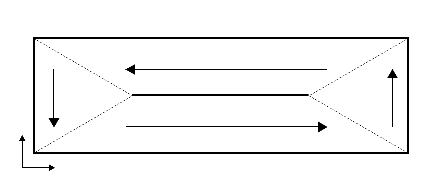
\includegraphics[width=\columnwidth]{pic01.eps}
		\caption{非対称Bloch磁壁の磁化構造}
		\label{fig04_1}
	\end{subfigure}
	\begin{subfigure}{0.8\columnwidth}
		\centering
		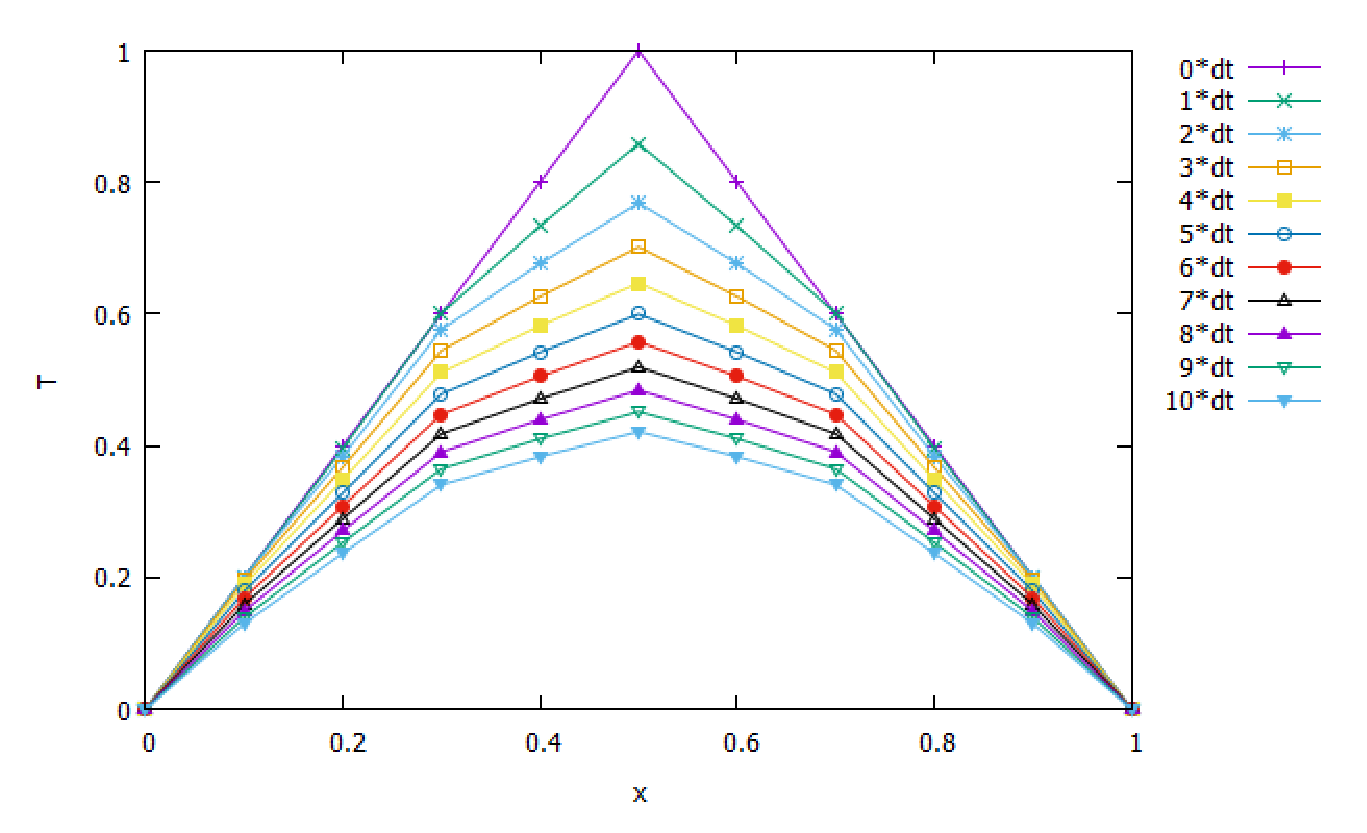
\includegraphics[width=\columnwidth]{pic02.eps}
		\caption{対称Bloch磁壁の磁化構造}
		\label{fig04_2}
	\end{subfigure}
	\caption{計算によって得られたBloch磁壁の磁化構造}
	\label{fig06}
\end{figure}

\begin{figure}[H]
	\centering
	\begin{subfigure}{0.8\columnwidth}
		\centering
		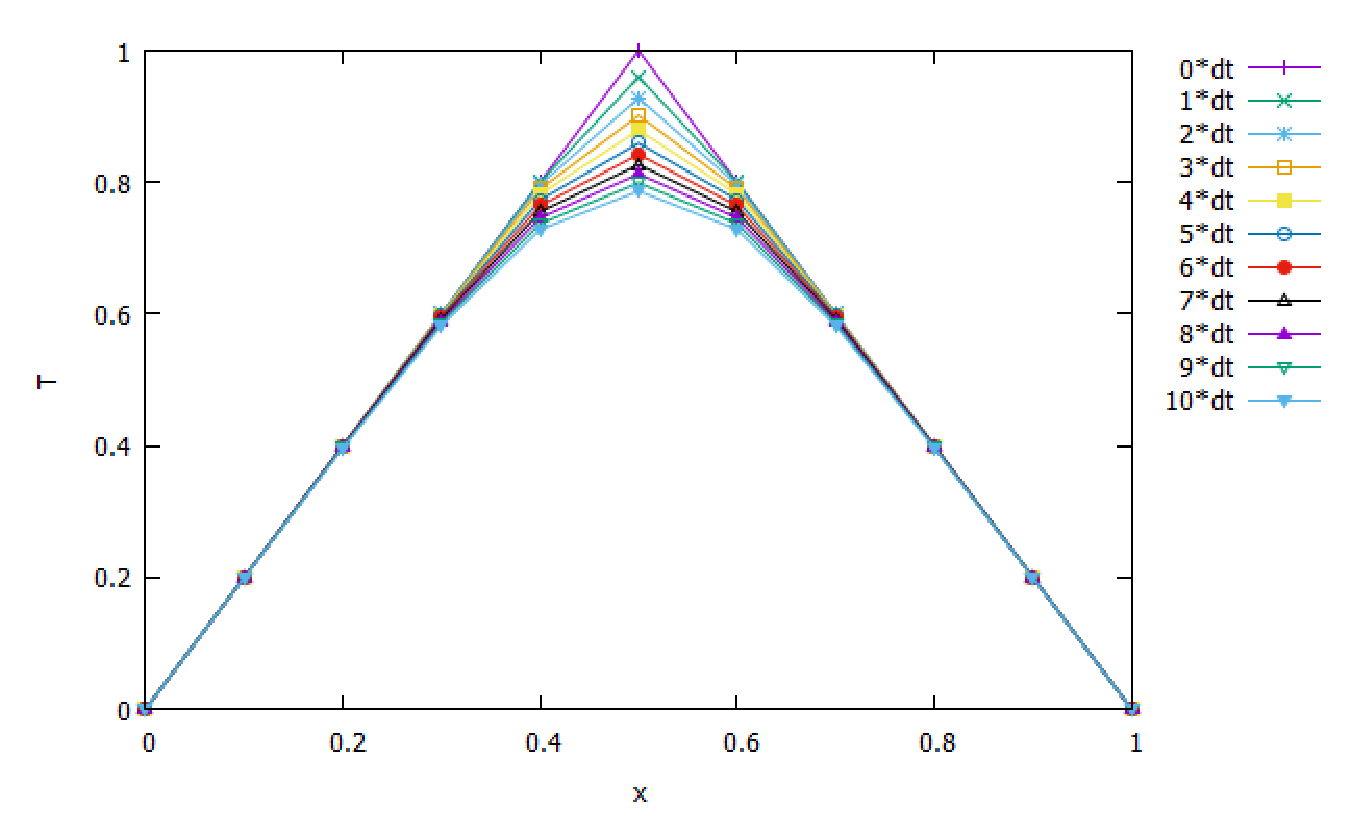
\includegraphics[width=\columnwidth]{pic03.eps}
		\caption{対称$\mathrm{N\Acute{e}el}$磁壁の磁化構造}
		\label{fig04_3}
	\end{subfigure}
	\begin{subfigure}{0.8\columnwidth}
		\centering
		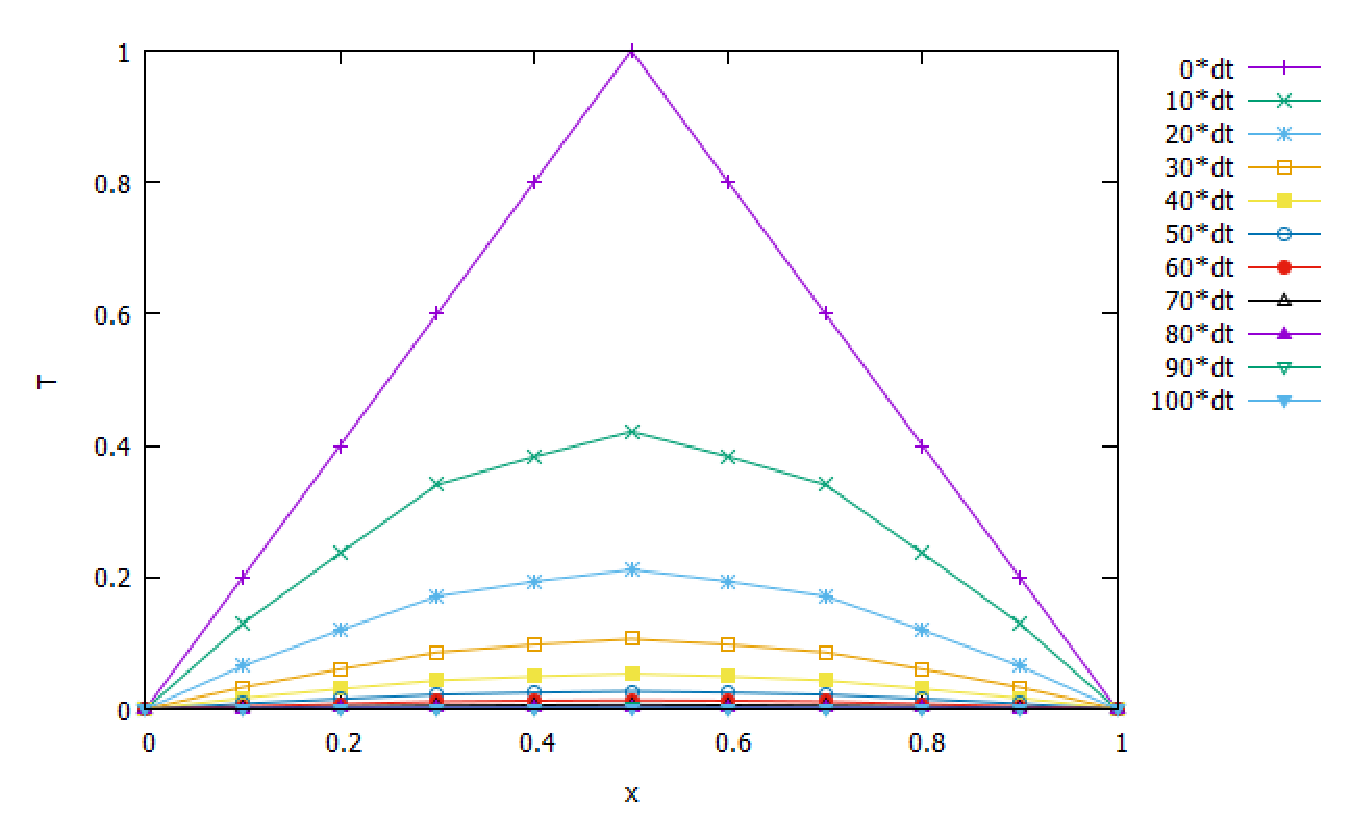
\includegraphics[width=\columnwidth]{pic04.eps}
		\caption{非対称$\mathrm{N\Acute{e}el}$磁壁の磁化構造}
		\label{fig04_4}
	\end{subfigure}
	\caption{計算によって得られた$\mathrm{N\Acute{e}el}$磁壁の磁化構造}
	\label{fig04}
\end{figure}

図\ref{fig06},\ref{fig04}からいくつかわかったことがある。
まず、対称非対称に限らず、Bloch磁壁は図\ref{fig01}の概念図と非常に近い形で計算がされた。
しかしながら、$\mathrm{N\Acute{e}el}$磁壁に関しては、対称非対称の双方で概念図と離れた形の計算結果となった。

さらには、図\ref{fig04_4}ではおおよそ$\mathrm{N\Acute{e}el}$磁壁とは見えるが、対称Bloch磁壁のような形とも捉えられる。
推察するに、膜厚がちょうど$\mathrm{N\Acute{e}el}$磁壁ともBloch磁壁とも成りきれない厚さだったからと捉えられる。
これは非対称$\mathrm{N\Acute{e}el}$磁壁が出現する条件と一致するが、計算結果自体は明らかに$\mathrm{N\Acute{e}el}$磁壁と、
判ずるのが難しいものとなった。

\subsection{小問4}
この小問では、計算点と計算時間の関係をグラフで示す。
該当のグラフは図\ref{fig05}としてまとめた。
\begin{figure}[H]
	\centering
	\includegraphics[width=14cm]{pic12.eps}
	\caption{計算点数と計算時間の関係のグラフ}
	\label{fig05}
\end{figure}

この図\ref{fig05}から、計算時間はnzの二乗に比例して増加していることが分かる。


\section{参考文献}
\begin{itemize}
  \item 配布されたテキスト
\end{itemize}

\end{document}